% %******************************************************************************
% % % introduction.tex %
% %******************************************************************************
% % % Title......: Introduction % % Author.....: GSCAR-DFKI % % Started....: Nov
% 2013 % % Emails.....: alcantara@poli.ufrj.br elael@poli.ufrj
% renan028@gmail.com % % Address....: Universidade Federal do Rio de Janeiro %  
%            Caixa Postal 68.504, CEP: 21.945-970 %              Rio de Janeiro,
% RJ - Brasil.
% %
% %******************************************************************************


% %******************************************************************************
% % SECTION - Eletronica
% %******************************************************************************

\section[Proposta 1 – Placa com Microcontrolador e Gateway Ethernet]{Proposta 1
– Placa com Microcontrolador e \\Gateway Ethernet}

\subsection{Arquitetura da Eletrônica Proposta 1 - versão 1}
A eletrônia é composta pelos seguintes dispositivos:
\begin{itemize}
  \item Dois Encoders da IFM: 24V e interface CAN. Datasheet em Anexo 1.
  \item Um sonar Super SeaKing da Tritech: 24V e interface RS232. Data\-sheet em
  Anexo 1
  \item Um Sistema Pan \& Tilt da Kongsberg: 24V e interface RS232. Data\-sheet
  em Anexo 1.
  \item Dois sensores Indutivos da Pepperl-Fuchs: 24V e saída ana\-lógico.
  Data\-sheet em Anexo 1.
  \item Um sensor de inclinação da IFM: 24V e saída analógica.
  Data\-sheet em Anexo 1.
  \item Um sensor de pressão da Velki: 24V e saída RS485. Datasheet em Anexo 1.
\end{itemize}

A placa com microcontrolador deve ter disponível todas as alimentações elétricas
e interfaces de comunicação descritas acima, além de saída Ethernet para
comunicação com a base. Na figura~\ref{placa}, pode ser observado o modelo 3D da
placa. Na figura~\ref{com_placa} e figura~\ref{alimentacao_placa}, são
representados os diagramas de interfaces de comunicação e alimentação elétrica,
respectivamente, do sistema. A seguir, será feita uma breve explicação dos
principais componentes da placa.

O microcontrolador AT90CAN64 será responsável pelo monitoramento e controle da
alimentação elétrica de todos os dispositivos, além de ser o respon\-sável pela
comunicação CAN com o Encoder.

O gateway Ethernet SR01E12 possui interfaces UART e analógicas. Des\-sa forma,
diversos dispositivos podem se conectar ao gateway atra\-vés de chips MAX232 ou
MAX485, que realizam a conversão RS232 ou RS485 para UART, respectivamente.

\begin{figure}[H]
\centering
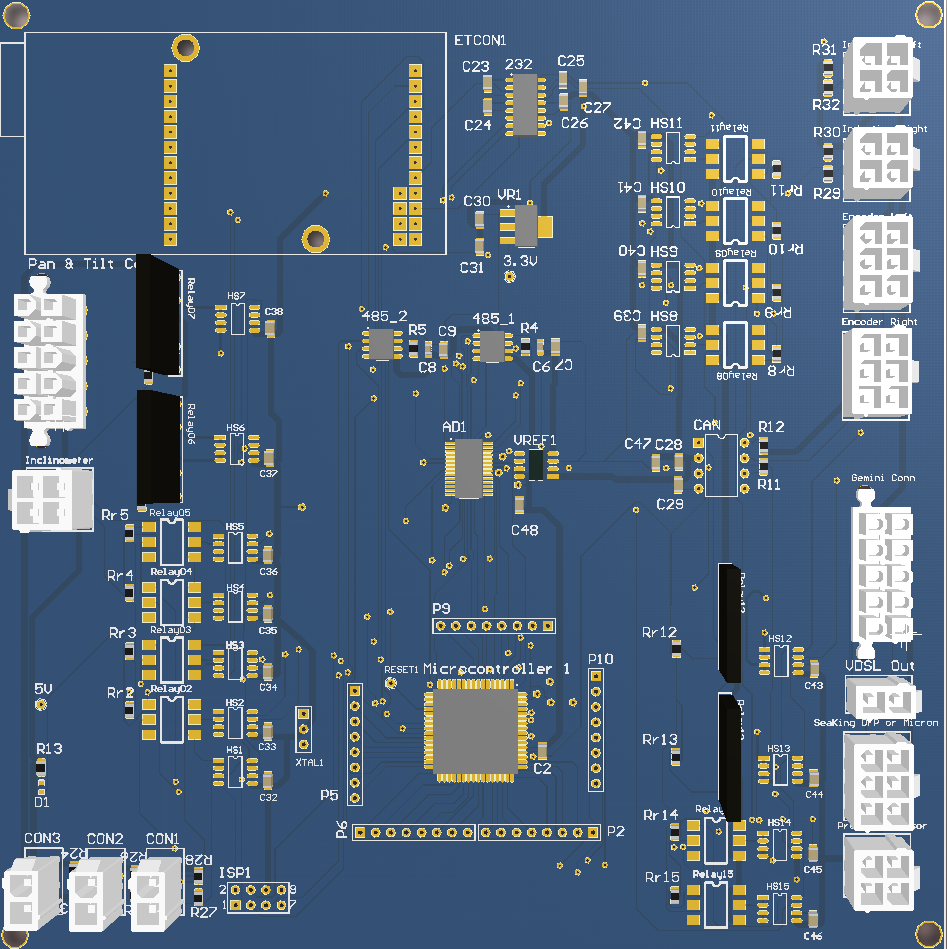
\includegraphics[width=1\columnwidth]{figs/eletronica/placav1.png}
\caption{Placa 3D}
\label{placa}
\end{figure}

\begin{figure}[H]
\centering
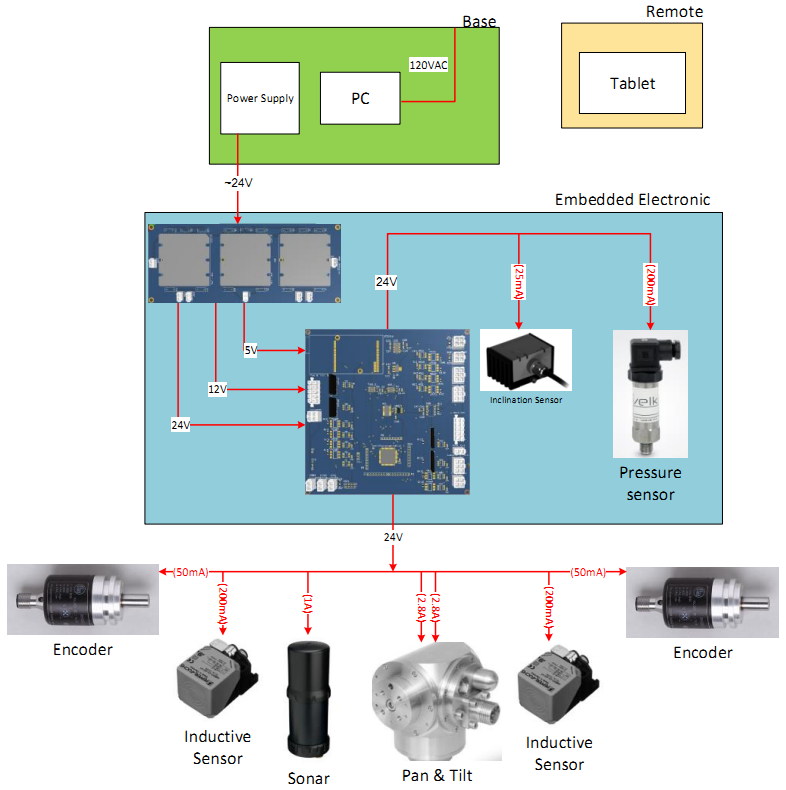
\includegraphics[width=1\columnwidth]{figs/eletronica/alimv1.png}
\caption{Diagrama de Alimentações}
\label{alimentacao_placa}
\end{figure}

\begin{figure}[H]
\centering
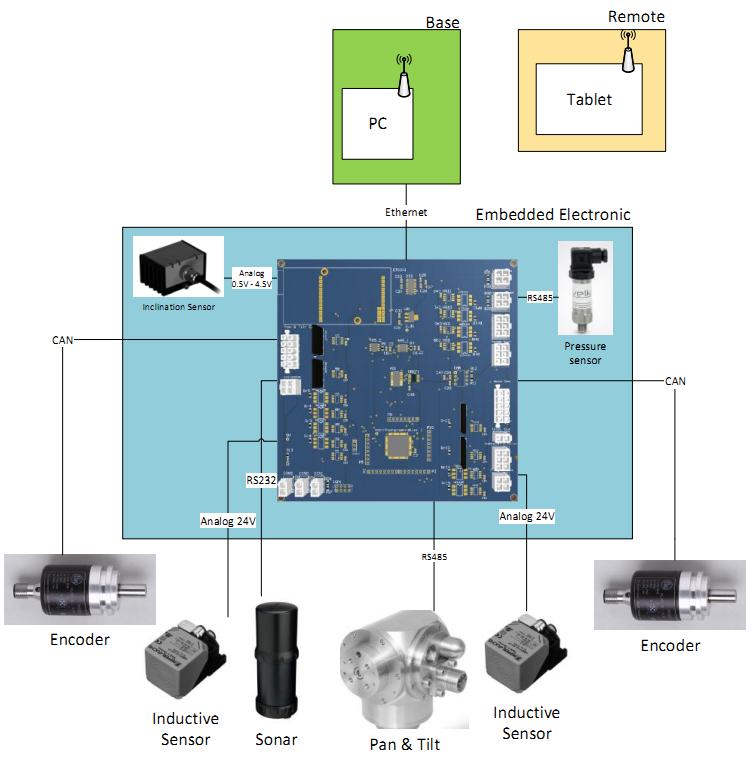
\includegraphics[width=1\columnwidth]{figs/eletronica/comv1.png}
\caption{Diagrama de Comunicação}
\label{com_placa}
\end{figure}

A placa com microcontrolador é uma solução de baixo custo, porém exige maior
tempo de execução. Há a necessidade de fabricação, montagem, testes elétricos e
lógicos da placa e programação de microcontrolador para gerenciamento de cada
interface, como o protocolo CANOpen.
A eletrônica deverá ser acoplada ao Lifting Beam, logo deverá ser construída uma
estrutura mecânica à prova d’água para esta solução.

\subsection{Arquitetura de Software Proposta 1 - versão 1}
O sistema se divide em três grandes blocos que serão encapsulados separadamente
e se comunicarão entre si, figura \ref{fig:FL:1}. A primeira parte consiste no
sistema de eletrônica embarcada composta pelos sensores e um equipamento de
roteamento dos dados (raias \emph{Sensores}, \emph{Conversores UART} e
\emph{Interface de Telemetria} da figura), a segunda parte consiste no sistema
de gerenciamento e processamento de dados em terra (raia \emph{Computação em
Terra}) e, finalmente, o último bloco consiste na camada de interface
homem-máquina , que consiste em um Tablet com sistema operacional Android (raia
\emph{Interface com o usuário}).

\afterpage{
\begin{landscape}
\begin{figure}
\centering
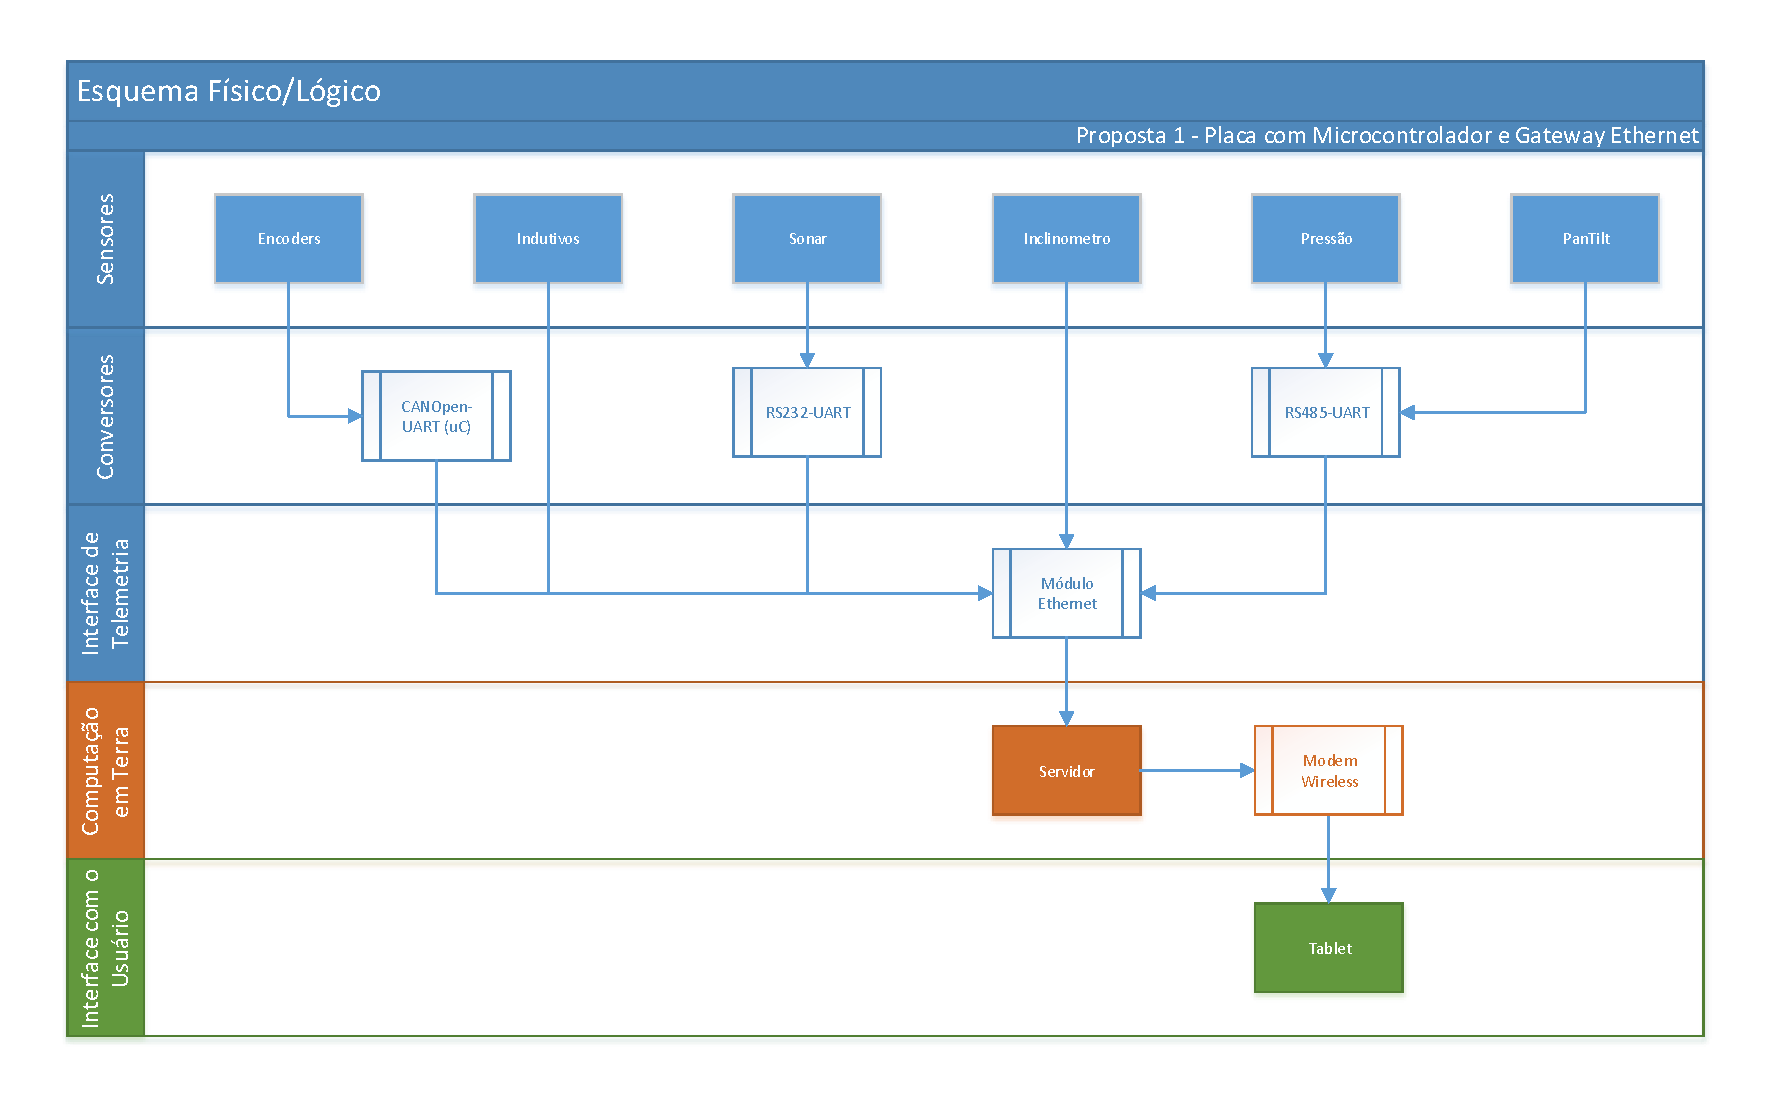
\includegraphics[width=1\linewidth,keepaspectratio]{figs/software/LogicoFisico/EsqLogicoFisico1n.pdf}
\caption{Relação entre os componentes físicos e as divisões lógicas da
proposta 1.}
\label{fig:FL:1}
\end{figure}
\end{landscape}
}

Cada sensor deverá possuir um driver para a interface entre o equipamento físico
e camada de software, isto é, os encoders, inclinômetro, os sensores indutivos e
o sensor de pressão possuirão drivers dedicados para a leitura de dados, feita
através de uma conexão Ethernet para a placa que interconecta os sensores. O
sonar e o módulo PanTilt também possuirão drivers próprios para a aquisição de
dados e controle.

Nesta proposta, após a aquisição de dados, a placa embarcada realizará o
roteamento e envio de todos os dados para o computador em terra por meio do
driver do módulo Ethernet.  Os dados transmitidos pela eletrônica embarcada são
separados em dois grandes grupos: referentes à Monitoração e os referentes à
Visualização Sonar.

No computador localizado em terra, figura \ref{fig:ES:1}, o componente de
software responsável pela monitoração irá processar e conformar os dados
provenientes dos sensores utilizados para o monitoramento das operações de
inserção e remoção (encoders, inclinômetro, sensores indutivos e sensor de
pressão). Os dados provenientes do sonar devem ser integrados com a posição do
elemento PanTilt, no componente Sonar-PanTilt, para que sejam consistentes e
completos.  O módulo de Reconstrução 3D é responsável, então, por traduzir os
dados processados pelo componente anterior em uma visualização inteligível para
o ser humano.  Um componente de segurança também é adicionado para monitorar a
correta utilização do sonar (apenas embaixo d’água), conferindo uma maior
robustez ao sistema.

\begin{figure}[H] 
\centering
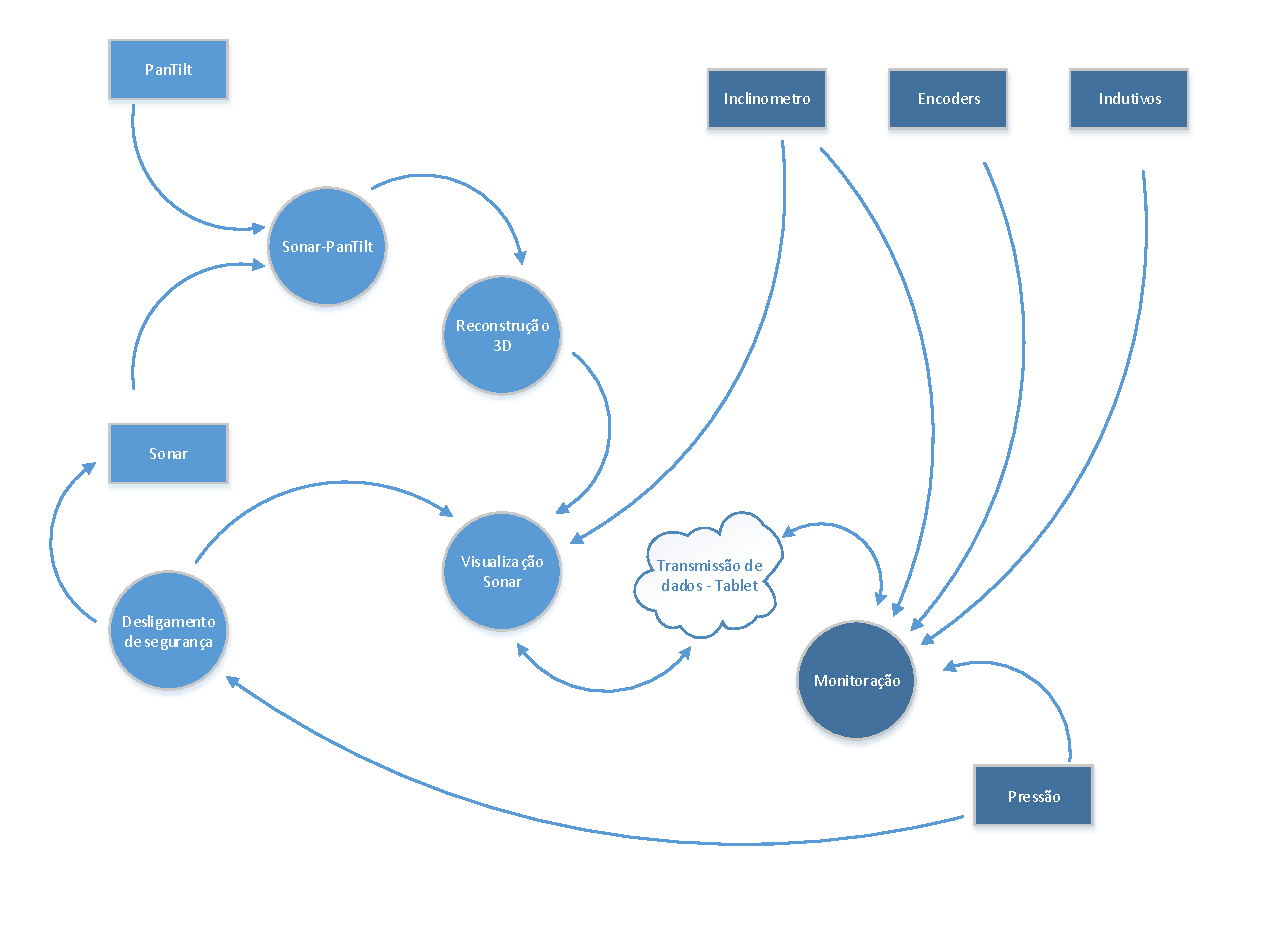
\includegraphics[width=\textwidth,height=\textheight,keepaspectratio]{figs/software/EstrutSoft/prop1_soft_2.pdf}
\caption{Interconexões entre os componentes de software da proposta 1.}
\label{fig:ES:1}
\end{figure}

Ambos os componentes de processamento e conformação de dados, Monitoração e
Visualização Sonar, irão se comunicar com o Tablet com sistema operacional
Android por meio do componente Transmissão de dados – Tablet, enviando os dados
processados e recebendo os comandos de controle.  A interface homem máquina
consiste em um aplicativo cuja finalidade é realizar a interface do sistema com
o usuário, possibilitando uma correta e fácil visualização de todas as
informações pertinentes do sistema e suas operações.

\subsection{Arquitetura da Eletrônica Proposta 1 - versão 2}
Após a primeira viagem técnica para Jirau em Maio/2014, houve algumas alterações
na arquitetura da eletrônica. 
A nova arquitetura da eletrônia é composta pelos seguintes dispositivos:
\begin{itemize}
  \item Dois Encoders da IFM: 24V e interface CAN. Datasheet em Anexo 1.
  \item Um sonar Super SeaKing da Tritech: 24V e interface RS232. Data\-sheet em
  Anexo 1
  \item Um Sistema Pan \& Tilt da Kongsberg: 24V e interface RS232. Data\-sheet
  em Anexo 1.
  \item Três sensores Indutivos da Pepperl-Fuchs: 24V e saída ana\-lógico.
  Data\-sheet em Anexo 1.
  \item Quatro sensor de inclinação da Pepperl-Fuchs: 24V e saída analógica.
  Data\-sheet em Anexo 1.
  \item Um sensor de pressão da Velki: 24V e saída RS485. Datasheet em Anexo 1.
\end{itemize}
Os sensores de inclinação acrescentados podem substituir os encoders, em caso de
restrição de acoplamento mecânico na viga pescadora. 
Os sensores de inclinação serão acoplados da mesma
maneira que os sensores indutivos

A placa com microcontrolador é semelhante à desenvolvida na versão 1,
acrescida de quatro conectores para os sensores de inclinação e mais um
conector para o sensor indutivo extra. 

O microcontrolador AT90CAN64 será responsável pelo monitoramento e controle da
alimentação elétrica de todos os dispositivos, além de interpretar os dados dos
quatro sensores de inclinação e se comunicar com o gateway Ethernet. 

Os sensores de inclinação adicionais podem substituir os encoders, em caso de
restrição de acoplamento mecânico na viga pescadora. Eles têm saída
analógica, que é interpretada pelo microcontrolador. Duas placas foram
desenvolvidas:~\ref{placav21} e ~\ref{placav22}, onde a segunda apresenta
amplificadores para condicionamento dos sinais analógicos provenientes dos
sensores de inclinação a fim de reduzir ruídos. Na
figura~\ref{com_placav2} e figura~\ref{alimentacao_placav2}, são
representados os diagramas de interfaces de comunicação e alimentação elétrica,
respectivamente, do sistema. A seguir, será feita uma breve explicação dos principais componentes da placa.

O gateway Ethernet SR01E12 possui interfaces UART e analógicas. Des\-sa forma,
diversos dispositivos podem se conectar ao gateway atra\-vés de chips MAX232 ou
MAX485, que realizam a conversão RS232 ou RS485 para UART, respectivamente.

\begin{figure}[H]
\centering
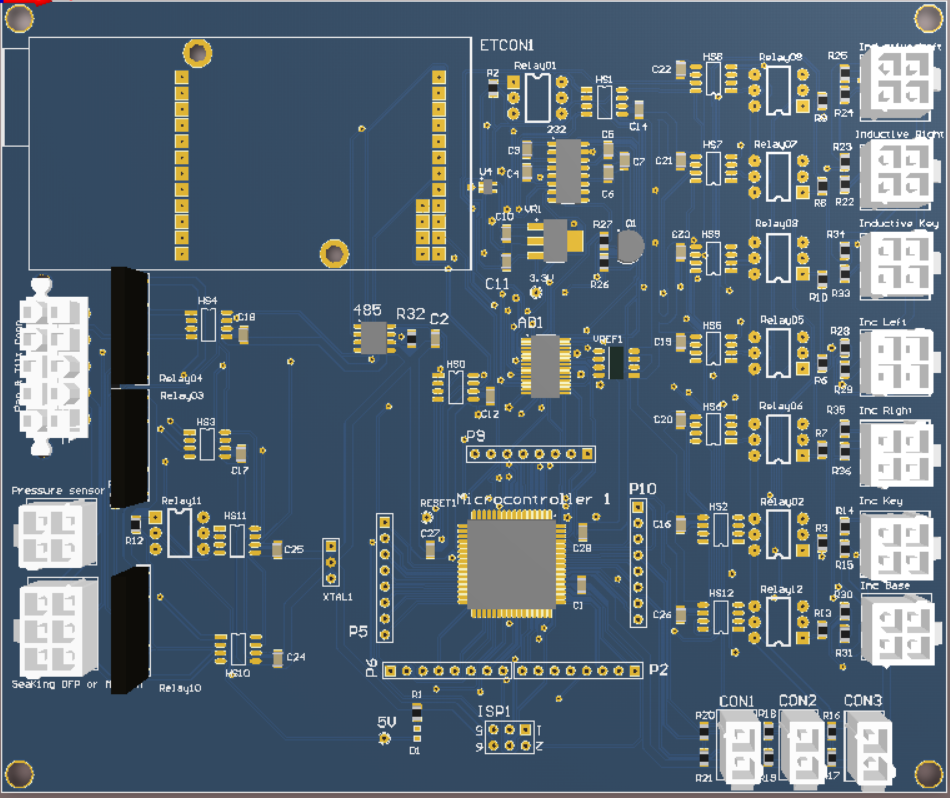
\includegraphics[width=1\columnwidth]{figs/eletronica/placav21.png}
\caption{Placa 3D - versão com sensores de inclinação sem condicionamento de
sinal}
\label{placav21}
\end{figure}

\begin{figure}[H]
\centering
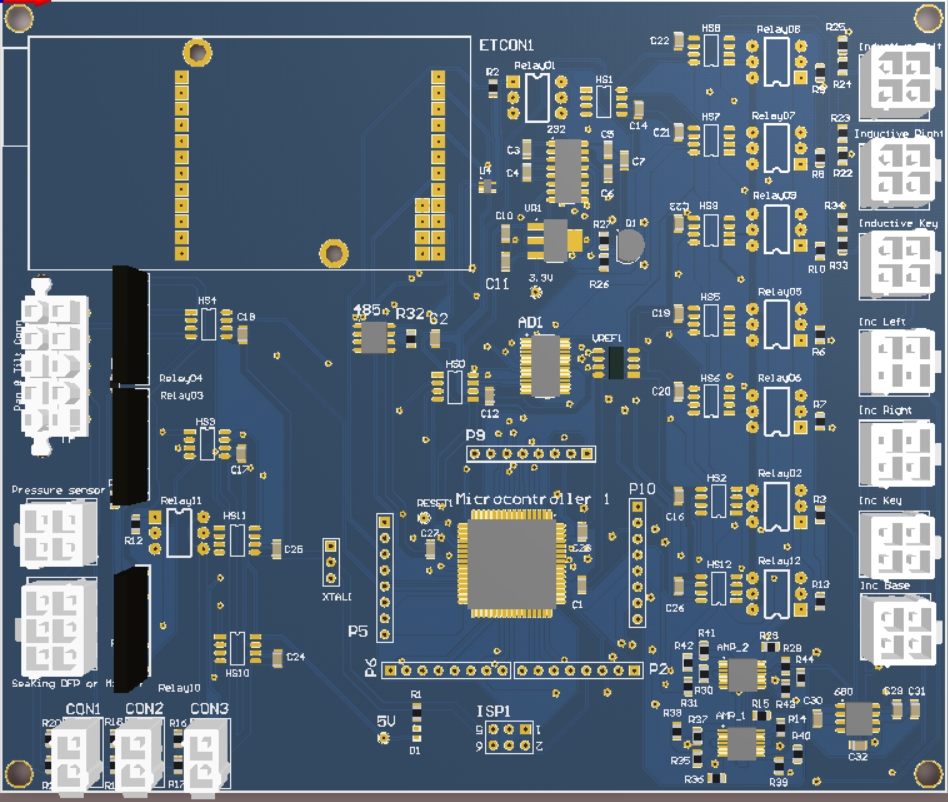
\includegraphics[width=1\columnwidth]{figs/eletronica/placav22.png}
\caption{Placa 3D - versão com sensores de inclinação com condicionamento de
sinal}
\label{placav22}
\end{figure}

\begin{figure}[H]
\centering
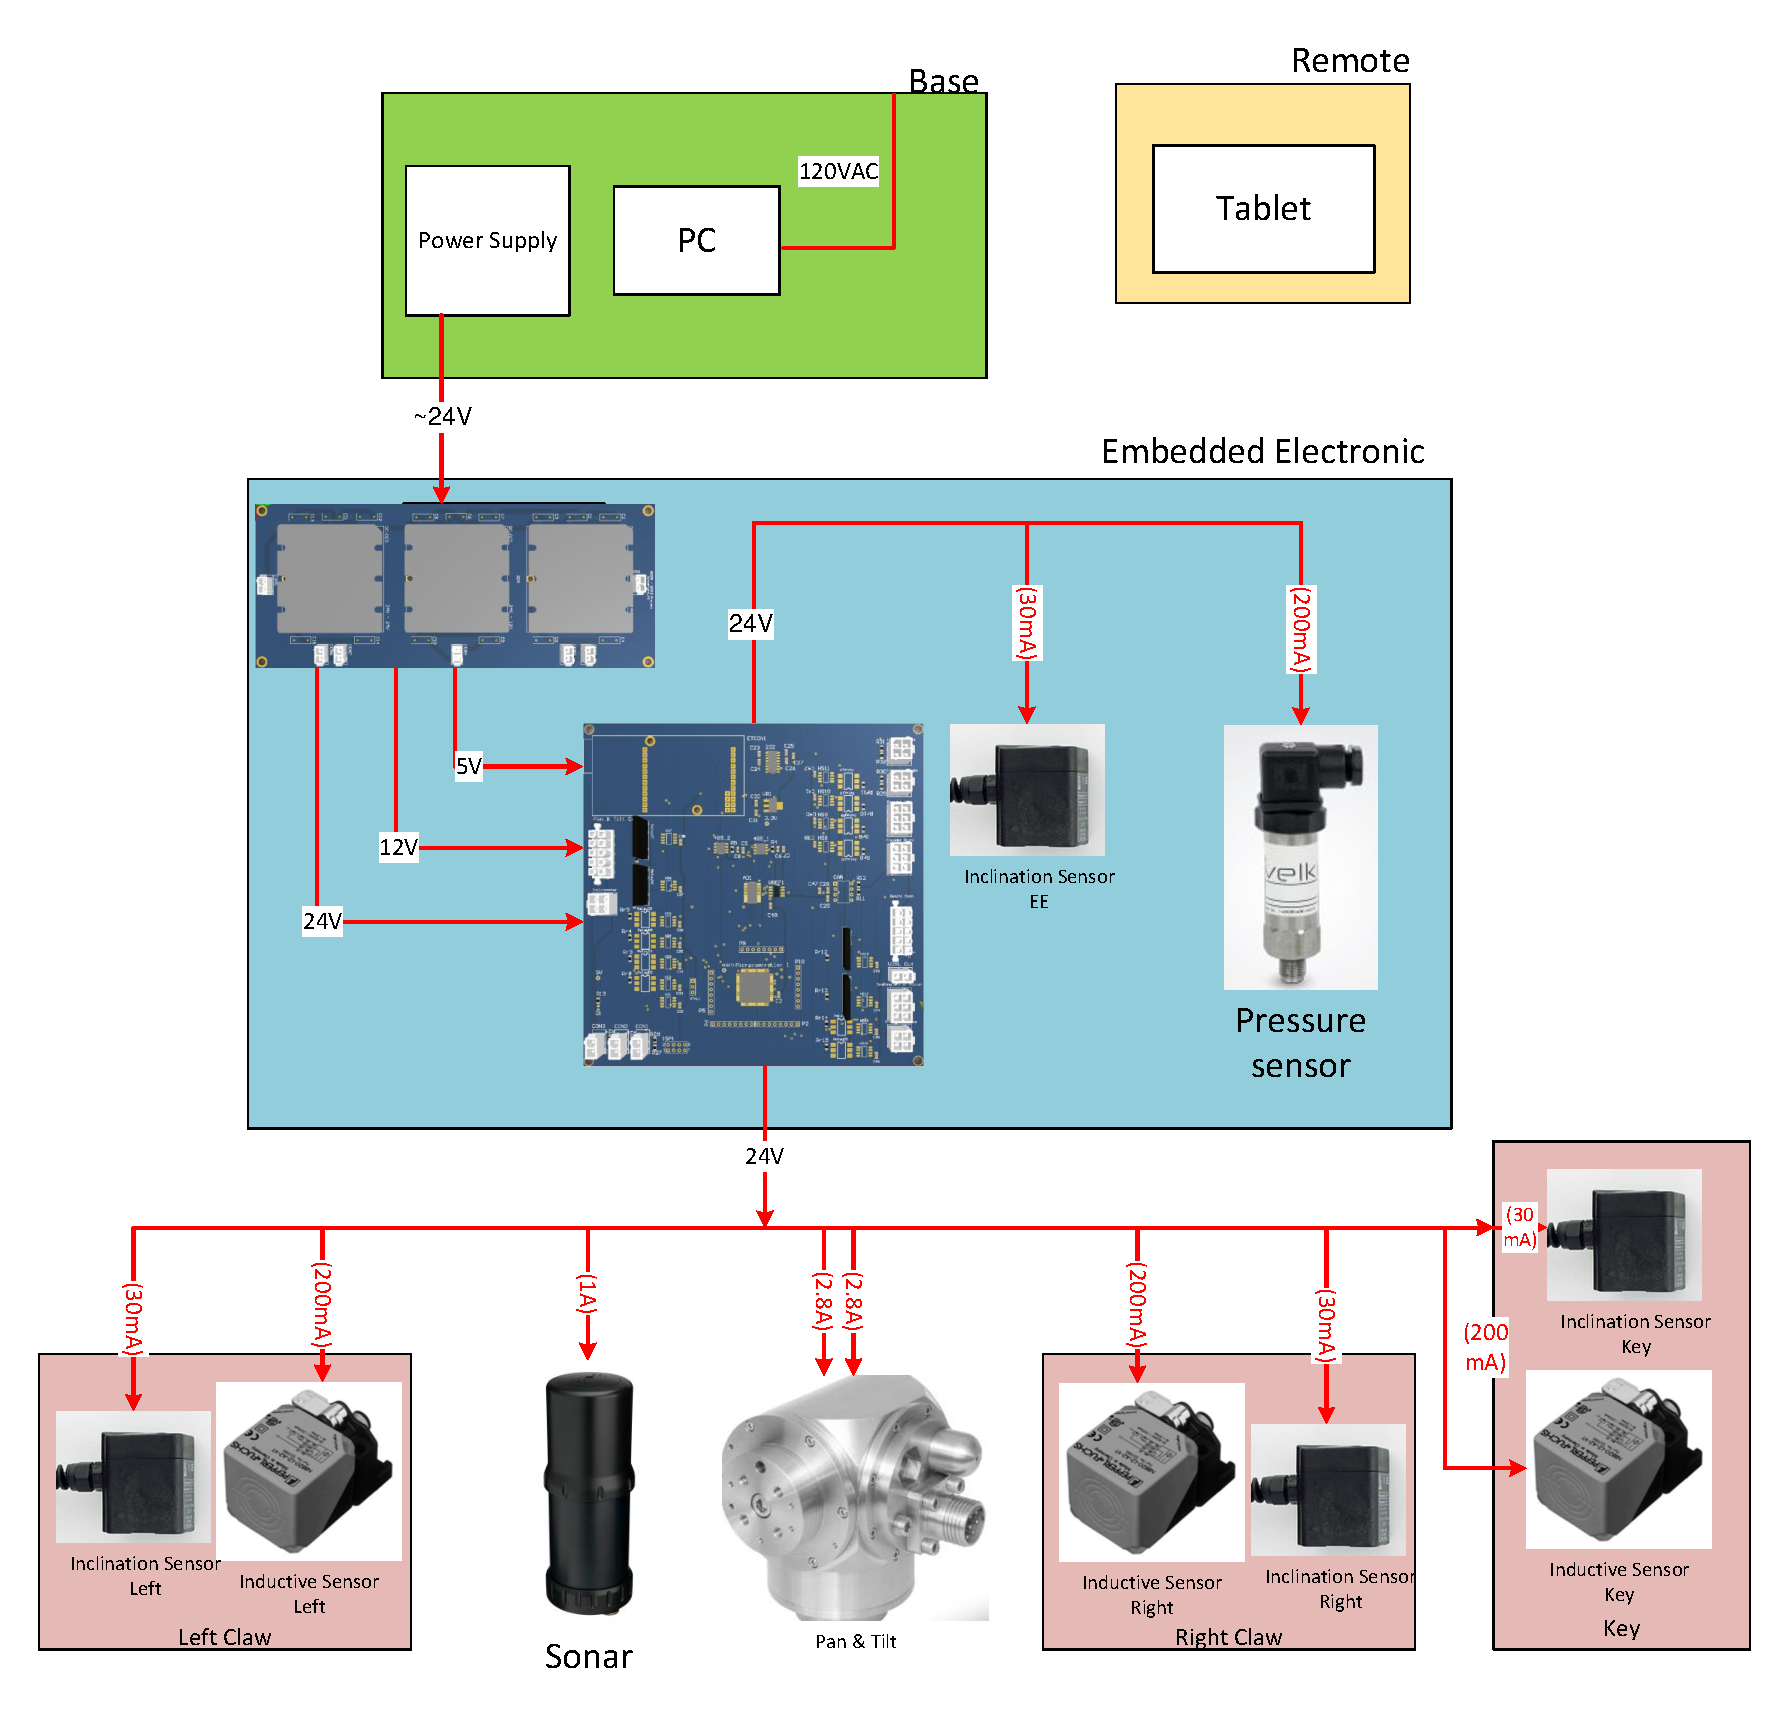
\includegraphics[width=1\columnwidth]{figs/eletronica/alimentacao_placav2.pdf}
\caption{Diagrama de Alimentações}
\label{alimentacao_placav2}
\end{figure}

\begin{figure}[H]
\centering
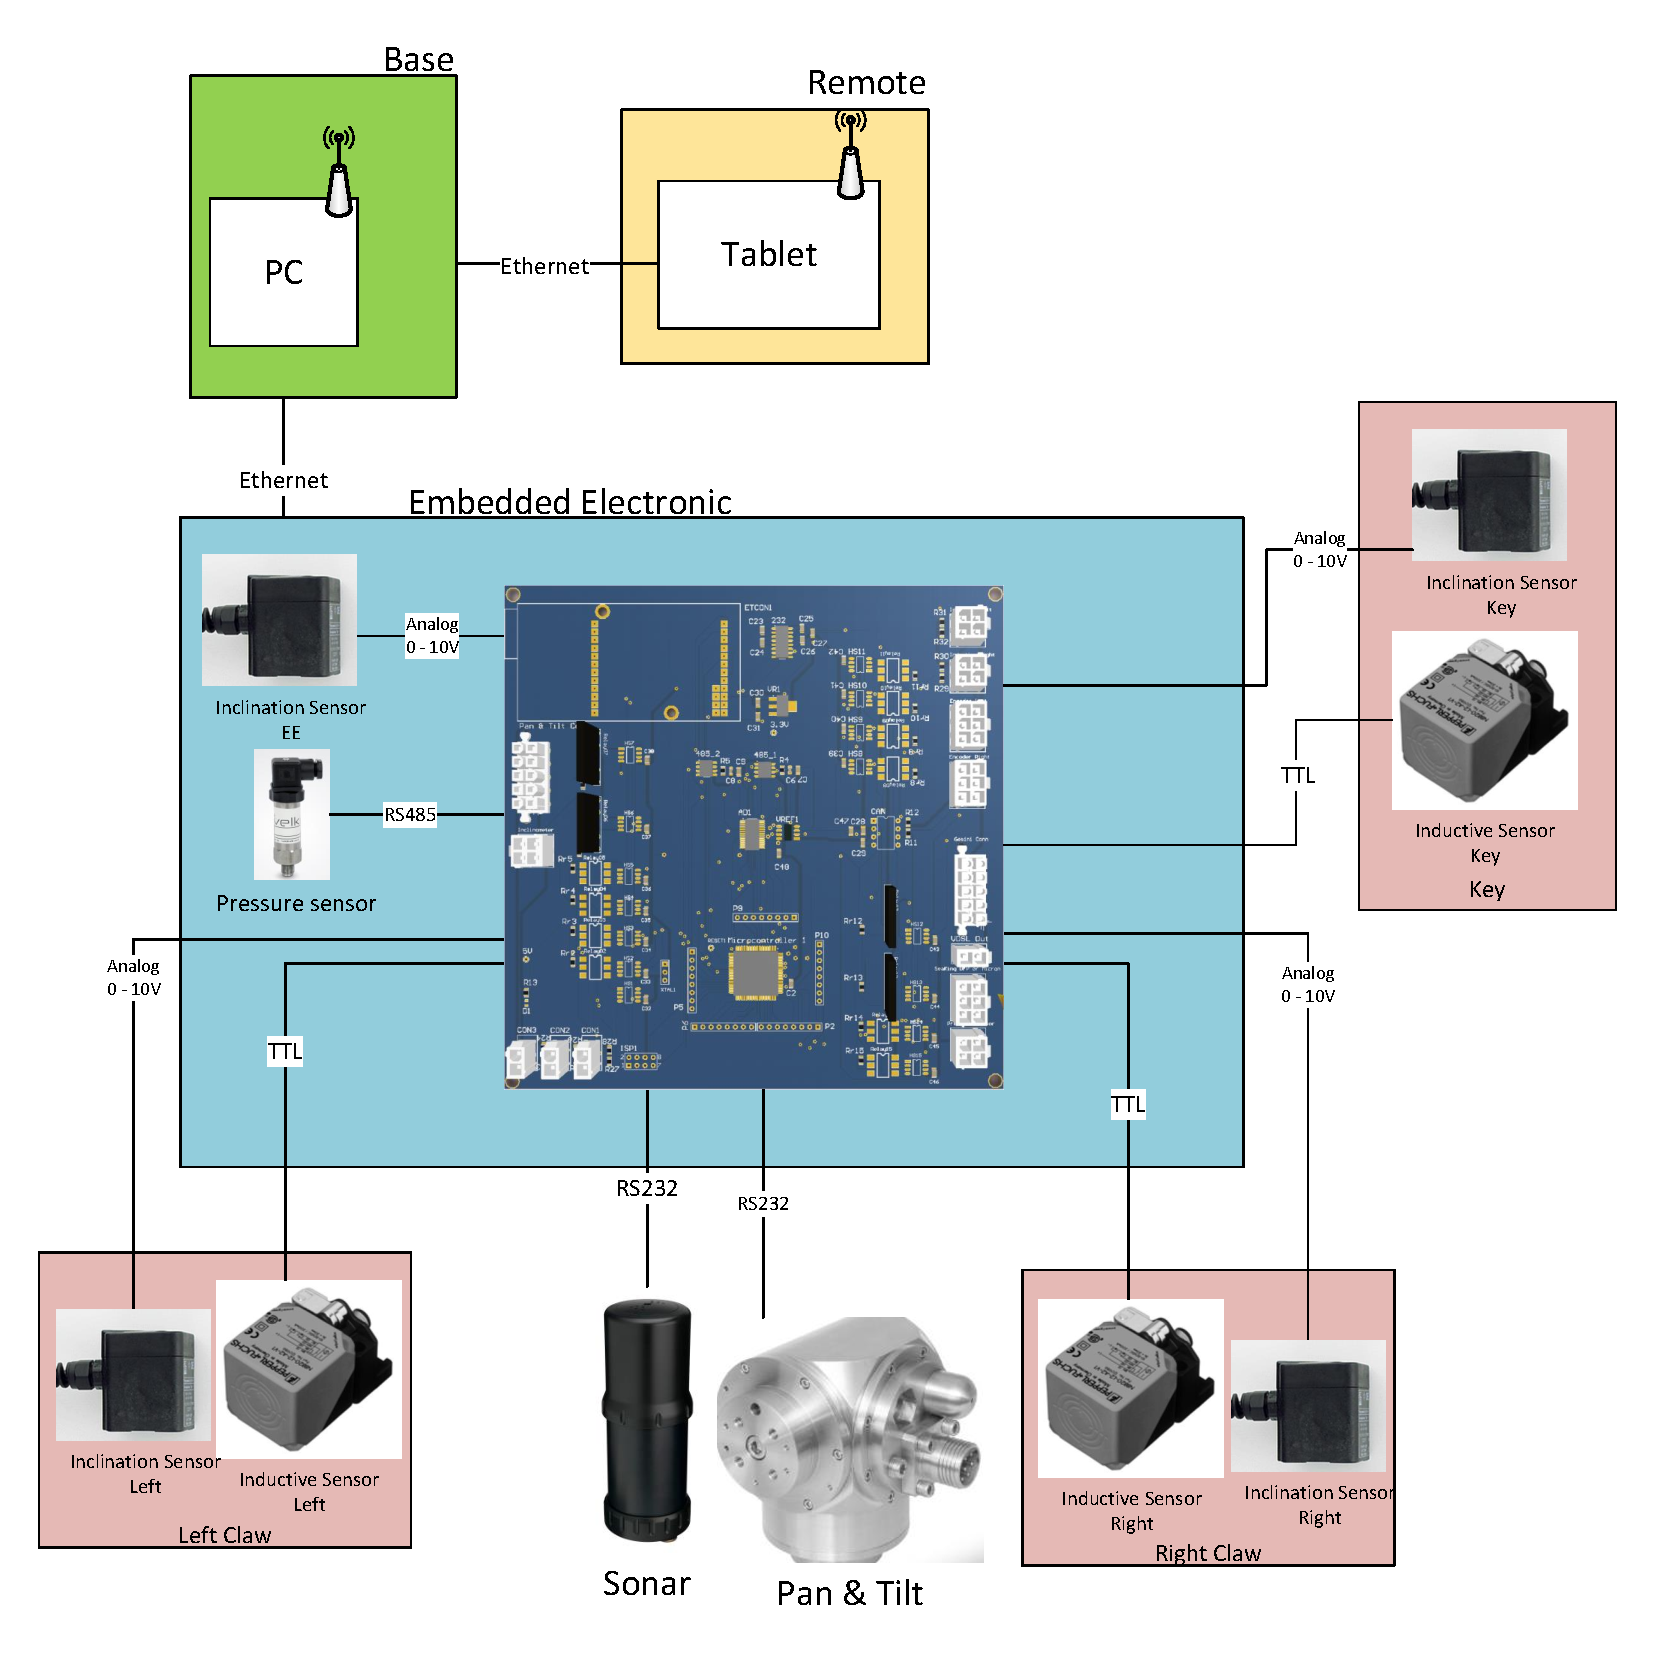
\includegraphics[width=1\columnwidth]{figs/eletronica/com_placav2.pdf}
\caption{Diagrama de Comunicação - versão 2}
\label{com_placav2}
\end{figure}